\documentclass[conference,10pt]{IEEEtran}
\IEEEoverridecommandlockouts
% The preceding line is only needed to identify funding in the first footnote. If that is unneeded, please comment it out.
\usepackage{cite}
\usepackage{amsmath,amssymb,amsfonts}
\usepackage{algorithmic}
\usepackage{graphicx}
\usepackage{textcomp}
\usepackage[T1]{fontenc}
\usepackage{mathptmx}
\def\BibTeX{{\rm B\kern-.05em{\sc i\kern-.025em b}\kern-.08em
		T\kern-.1667em\lower.7ex\hbox{E}\kern-.125emX}}
\begin{document}

	\title{Solving Multiplayer Snake using Competitive Self-play Reinforcement Learning}

	\author{\IEEEauthorblockN{Nitish Kumar Rath}
		\IEEEauthorblockA{\textit{University  of Florida}\\
			nitish.rath@ufl.edu}
		\and
		\IEEEauthorblockN{Sourav Dutta}
		\IEEEauthorblockA{\textit{University of Florida}\\
			duttasourav@ufl.edu}
		\and
		\IEEEauthorblockN{Srajan Paliwal}
		\IEEEauthorblockA{\textit{University of Florida}\\
			srajanpaliwal@ufl.edu}
	}

	\maketitle

	\begin{abstract}
		This project aims at solving one of the open research problems published by OpenAI\cite{n3}. This project is focused on implementing a multi-player clone of a Snake game based on the online hit \textit{slither.io}. The project aims to explore various reinforcement learning methodologies to solve the problem. This makes use of Gym toolkit by openAI as a base for reinforcement learning.  Further we want to see how to control the behaviour of the snakes by changing the reward structures, viz., competitive and co-operative. The project also aims at making the game environment a bit more complex than to see the effect of techniques like transfer learning and curriculum learning. 
	\end{abstract}

	\begin{IEEEkeywords}
		deep learning, reinforcement learning, Multi-Agent, Transfer Learning, Agent Behavior
	\end{IEEEkeywords}

	\section{Introduction}
	Recently we have seen a rise in controlling agents using deep reinforcement learning directly from high-dimensional inputs. The inputs could be vision or speech or both combined. These are steps toward
	general artificial intelligence and these methods are directly applied to
	learn self play such as Alpha Go \cite{sp9} Atari \cite{sp3}. It has become
	evident that such algorithms achieve good performance on difficult problems
	without problem specific engineering. Also, it has been observed that the
	strategies are more complex than the environment. With traditional RL the
	rewards for a step were immediately available, but with games there can be
	complex strategies as the rewards can be a result of several consecutive steps.
	These methods use a wide variety of techniques like Markov decision process,
	discounted future reward, Q-learning \cite{sd5} and Policy gradient \cite{sd4}.\break
	This proposal aims at solving a multi-player snake game proposed by OpenAI as a open research topic and inspired by
	\textit{slither.io} \cite{sd2} where snakes consume food to increase length and
	kills other snakes. The game will be developed as a
	OpenAI Gym \cite{sd2} environment which provides an interface between the game
	and the learning algorithm. It allows developers to focus on the learning
	environment with much less stress on interacting with the game.
	
	
The project primarily uses Deep Q-Netowrks as agents to learn the environment and act. We have made use of techniques like transfer learning and curriculum learning to reuse the learned weights in a given set of constraints in another. We have experimented on the behaviour of the snakes by altering the reward structure. The behaviour we explored was competitive and co-operative. We have well documented our approach, key elements of our project and results in this report. 
	\section{Related Work}
	Watkins\cite{sp1} introduced Q- learning as a simple way for training agents to learn
	optimal policies for a Markov decision process. Then, Tan\cite{sp2} further extend
	this idea to multiagents, his paper demonstrated that
	multi-agents can learn cooperative behavior in a simulated social environment with reinforcement learning.

	In past couple of years, a combination of deep neural network, Q-learning and
	competitive self play has allowed researchers to train agents for a variety
	of complex tasks. DeepMind\cite{sp3} used CNN and Q-learning to train deep Q-neural
	network agent that achieved scores comparable to professional human game
	testers in 49 Atari games. This was the first example of an AI algorithm
	that can excel at different tasks. DeepMind further improved DQN by introducing
	techniques like Double Q Learning\cite{sp4}, Prioritized Replay\cite{sp5}, Dueling DQN\cite{sp6}.  After
	that, Deep mind made a Go-bot\cite{sp7} based on a combination of deep Q-neural
	networks and tree search. It plays like a human player and can be compared to the top players. Neural networks were trained by supervised and reinforcement learning using human
	expert moves. The tree search algorithm
	combined neural network evaluations with Monte Carlo rollouts. In 2017, Alpha
	Go zero\cite{sp8} introduced an algorithm that learns without any human inputs.
	This algorithm learns through reinforcement self-play from scratch i.e. it starts
	with random plays and keeps improving itself. The search algorithms to evaluate moves used a single
	neural network without Monte Carlo rollouts.

	OpenAI experimented with competitive and cooperative self-play\cite{sp9}. They simulated
	multiple 3D-multiagent environments and demonstrated that agents can learn
	complex skills in simple environments with simple rewards. OpenAI\cite{sp10} used
	self-play to create a Dota 2 bot that defeated professional players in a
	constrained 1v1 match.
	\break
	\break
	Tampuu, Matiisen et al\cite{sd7} explored multi-agent environments and observed how the agents performed based on the reward system. They performed the experiments on Pong game. The most interesting experiment which is relevant to our project is simulating a collaborative and competitive environment and observe how agents interact. In the work done by Tampuu, Matiisen et al\cite{sd3}, the player was rewarded when the opponent lost in a competitive environment, whereas in a collaborative environment both players we penalized when any one of them lost. They clearly observed different agent behavior for these cases.
	\break
	\break
	We would like to experiment this on a multi-agent snake game where the snakes can be rewarded not only on the amount of food consumed but how many snakes are alive at any given moment. In a collaborative environment the snakes should avoid killing other snakes and avoid death to consume the available food. However, in a competitive environment a snake should focus on how it is able to stay alive longer and consume more food.

\begin{figure*}[]
	
	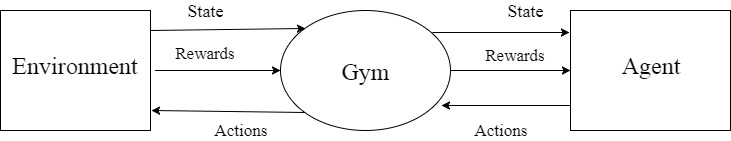
\includegraphics[width=\linewidth]{flow.jpg}
	\caption{Rough Flow of the algorithm}
	\label{sia}
	
\end{figure*}
\begin{figure*}[]
	
	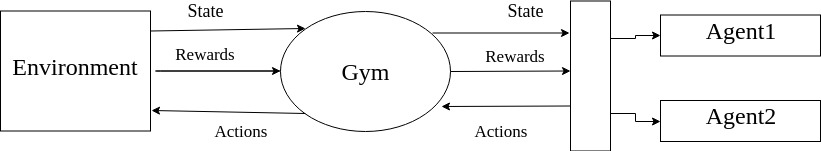
\includegraphics[width=\linewidth]{multi_agent.jpg}
	\caption{Rough Flow of the algorithm}
	\label{ma}
	
\end{figure*}
	\section{System Architecture}
		
	Our system consists of three major components: Interface, Environment and Agent, with Interface acting as the bridge between the game(Environment) and Agent(algorithm). Fig. \label{[sia]} shows our system architecture for the single player environment. For the multi-player version we added a wrapper on top the agents to function a interface between the environment and the agents. This was done inorder to preserve data flow sanity. The architecture for the multi-player system is given in Fig. \label{[ma]}

	\subsection{Interface}
	We are using OpenAI Gym\cite{sd3} as an Interface between the game and the training agent. OpenAI Gym provides APIs to interact with the game environment. It is a toolkit for developing and comparing reinforcement learning algorithms and provides some pre-built game environments to experiment with. For these games we can focus primarily on the algorithm and not worry about how the game works. Interactions with the game include initializing a game, ending or resetting the ongoing game and stepping through the game. The step function takes one action from a pre-defined set of actions called "action space". On completion of the step function, an "observation space" is returned. The observation space contains the game state after an action has been performed and varies from game to game. It can be as simple as the current game snapshot  or any complex data like coordinates and speed of each entity in the game. It also contains a reward for the current action taken and a flag which states whether the game ended or not.
	\subsection{Environment}
	\begin{figure}[]
		
		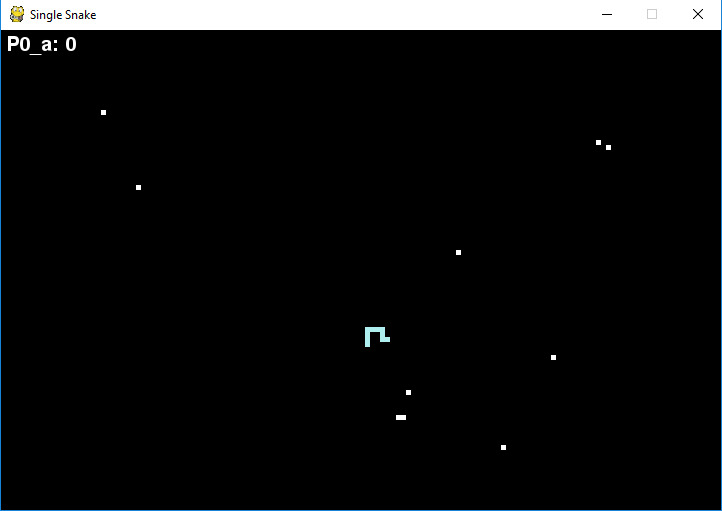
\includegraphics[width = \linewidth]{plot/single.jpeg}
		\caption{Snapshot of single player Environment}
		\label{se}
		
	\end{figure}
	\begin{figure}[]
		
		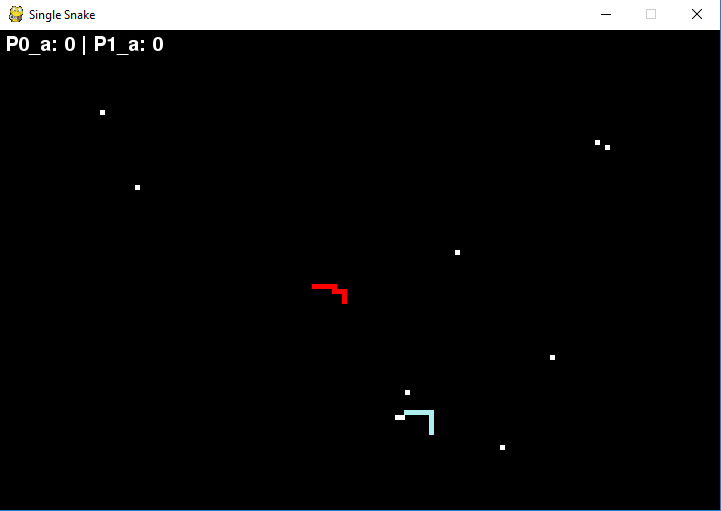
\includegraphics[width = \linewidth]{plot/multi.jpeg}
		\caption{Snapshot of multi player Environment}
		\label{me}
		
	\end{figure}
	The environment is the game that the agent tries to learn. Our first requirement was to build a snake game compatible with OpenAI Gym APIs. One of the snake game implementations which was similar to what we required was implemented by Loonride\cite{sd4}. We modified the game and added a layer on top of it to act as wrapper and make it compatible with Gym. The game was built in JavaScript using Phaser game engine. For the ease of use and make minimal changes we simulated the browser experience in a headless mode using selenium web driver.
	\break
	\break
	We modified the game to expose information like coordinates of the snakes, scores, whether the snakes is alive or not, food positions and the current game snapshot. This information is used by the agent algorithm to learn the game play. Furthermore, the input to the snake bot was also changed to take inputs from the action space instead of input devices such as mouse or keyboard.
	\break
	Upon training it was discovered that the process was too slow due to communication latencies in the selenium driver. Therefore, we moved to a simpler game environement, although this was a more realistic environment.The python game uses PyGame and is much faster than the JavaScript versoin. The snake in this case has less degrees of freedom. It can go either forward or turn left or right. It is a pixelated game where the entire game space can be consired as nxn blocks or big pixels and the snake can move one block at a time. Similarly the food is of size 1x1 block. We have two versions of the game. First, there is only one food and a new food appears randomly on the screen when it is consumed. In the second version there are more than one food. This game also runs on server in a headless or non-ui mode.
	
	After completing our tests on a single player snake game. We made some changes to the environment to adapt to a multi player game and made it more complex to make the agent learn complex environment.  We added a capability to spawn more than one snakes or agents which can be independently controlled by different algorithms. The environment takes an array of actions for each agent and executes it. Then it returns the state of the environment as an array for each agent. The evironment is sent with respect to each agent. The agent sees itself in one color and the other snakes are colored in red. This helps distinguish other players when the environment screenshot is sent. Before sending the data for a agent the canvas is redrawn with updated colors without executing any movement.
	\break
	\break
	We tried a windowed environment for out analysis. It is very similar to a real life scenario where the player is present in a large arena but is able to view only its surroundings. For each agent a small rectangular section is cropped and returned for training. The entire dimension is same as before which is 720px x 480px but the game objets and movements are scaled down four times. This increases the area but does not increase the actual number of pixels displayed. Pygame runs very slowly when a large number of pixels have to be updated at high frames per second. Keeping the number of pixels same allows us to run the pygame without increases any time for rendering. The window is of size 180px x 120px and does not change always as the agent moves. The window remains static unless the player moves to the edge of the window. Once the player moves towards the edge of the window, the window bounds are re-calculated according to the updated poisition of the player. This is done individually for each agent as each one of them sees their surrounding.
	\break
	\break
	The other change that we made in the environment was the reward structure. We added rewards for killing other snakes and dying. These rewards can be tweaked when the environment is instantiated. Using the different reards for killing the environment can be made cooperative or competitives. This way different agent behaviors can be learned.
	\break
	\break
	Sometimes, the snake is stuck in a loop while training. This affects training as the it does not add any new scenario to train. We added a max step count for the game to avoid such a scenario. Similarly, a max score was also added. The game stopped when any agent reached this score. This is to avoid the game to run infinitely since the food keeps appearing after consuming. 


	\subsection{Agent}
		\begin{figure}[]
			
			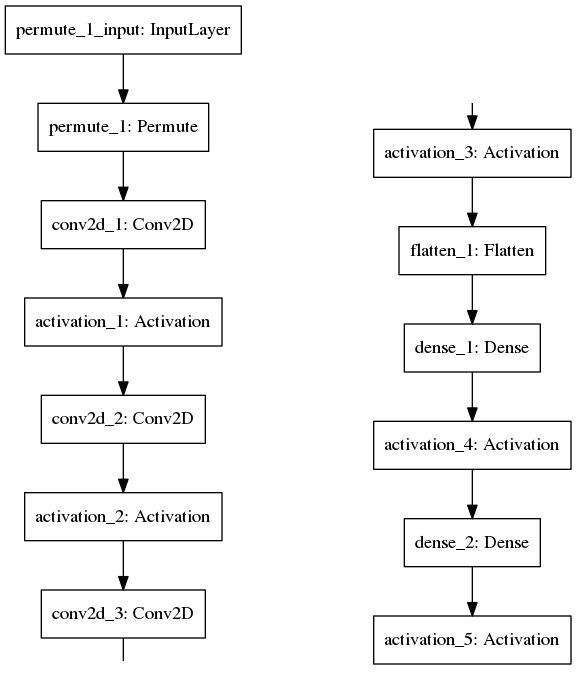
\includegraphics[scale=0.5]{model.png}
			\caption{Network Model}
			\label{model}
			
		\end{figure}
	The agent here is the algorithm that runs the players in the game. In our work we chose to use Q-learning, a form of reinforcement learning to figure out the game play by using the feedback provided by the game. Our training algorithm was inspired by Deep Q-learning technique proposed by DeepMind\cite{n4}.
	\break
	\break
	We made use of the Keras implementation of the Deep Q-learning developed by Matthias Plappert.\cite{n5}. This library also contains some other implementation of reinforcement algorithms like Double DQN and SARSA. It works with tensorflow backend and can be trained on a CPU and GPU and is also compatible with the APIs of OpenAI Gym.
	\break
	\break
	We made use of the network as proposed by DeepMind as a agent. Our network receives the game state and decides on a action. It then uses the feedback, rewards and observation pertaining to the action, from the game to backpropagate and approximates a Q-function for efficient game play.
	Figure\ref{model} shows the model that we implemented.
	\break
	\break
	For the single player environment, the game environment was modified and developed in a way to make it compliant with OpenAI Gym and the training functions in the Keras-RL implementation.
	\break
	\break 
	
	For the multi-player environment, using the same learning implementation would be difficulty. In order for the algorithm to run smoothly data flow sanity is essential. The observtaions and rewards of each each agent should be delivered to each agents learning algorithm for proper training. Hence an interface was built between OpenAI gym and the leaning algorithms. This interface took care of maintaining the data flow and proper running of the system. This new implementation was an extension of the Keras-RL implementation. Functionalities for proper logging, parsing observations and sending inputs to the network was implemented. 

	\section{Algorithms}
	Our work makes use of reinforcement learning, Q-learning to be specific to observe the game and approximate a appropriate function for game play. The following give details about the algorithm and policies used to train it.

	\subsection{Q-Learning}
	
	\begin{figure*}[]
		
		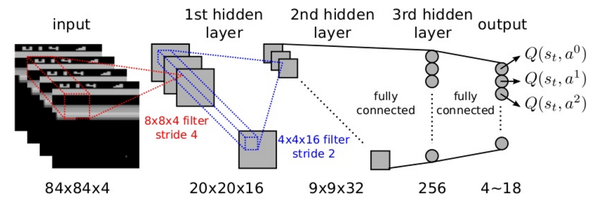
\includegraphics[width=\linewidth]{pmodel.png}
		\caption{Rough Flow of the algorithm}
		\label{pmodel}
		
	\end{figure*}
	Q- learning is a reinforcement learning technique where a function Q(s,a), where is the s is the present state and a is the action to be performed, is learnt to produce efficient actions for a given state s. The function is highly environment dependent and varies from environment to environment. 
	\break
	\break
	In simple words it gives the optimal score that can be gained in the current state so that the overall game score is maximum at the end of it. This means that the function must take in account the possible future rewards to determine an efficient action. To accomplish this, it must be aware of the rewards of all <s,a> pairs.
	\break
	\break
	 In simple game environment like tic-tac-toe, all <s,a> pairs can be listed in a table and Q-values updated to converge at a optimum point. In scenarios like atari games or Snake, the number of <s,a> pairs is too large to record. Also most of this may never be visited. Hence, DeepMind came up with a modified Q-learning technique, \textit{Deep Q-Networks}, based on Deep learning to efficiently approximate the Q-function. The algorithms works great for environments with a limited action state. 
	 \break
	 \break
	 The network architecture for the model is based on a CNN. This helps in identifying the image elements of the observation. In addition it uses a additional memory during training to store data/states-action experienced till now. It is refreshed so as to update the experiences with training. This helps in string state-action pairs with better Q-values. The algorithm, during training, takes a sample from this memory and calculates the future reward using a discount factor.
	 \break
	 \break
	  For testing however it does not need an additional memory. It determines action using solely the CNN. 

	\subsection{Exploration-Exploitation Dilemma}
	As discussed above, it is difficult to map all <s,a> pairs in complex game environments. There is always a dilemma between choosing a new action for a state to explore new states or going on with the previous learned actions to exploit more from the game play. Thus there has to be a effective trade-off between the two for learning the game optimally. DeepMind came up with policies to deal with this. Our work implements them and gives a comparative result.
	\break
	\break
	One such policy is \( \epsilon \)GreedyPolicy . This is a improvement on greedily choosing a know <s,a> pair. In this the algorithm may choose to take a new action based on a probability defined by  \( \epsilon \). The algorithm chooses to take a action inorder to exploit the game but may choose to take a explorative action the game depending on the probability.
	\break
	\break
	Another such policy is BoltzmannQpolicy, which is purely explorative. The policy chooses to takes an action based on the probability according to the predicted Q values.
	\break
	\break
	Usually, in practice, a explorative policy is chosen during training and a exploitative policy is chosen during testing.


	\section{Techniques for training Multi-agent}
	  In our multi-player snake environment,  the game field is only partially observable by a snake and food is sparsely scattered in the game field. This makes exploration harder as the snake won't receive a reward consistently and reliably. We realized this as we tried to train our agents from scratch is a complex environment. The snakes
	didn't even learn to collect food. The agent also took a lot of training time to come to converge as a sub-optimal solution. They mostly moved in a straight line and die by hitting a wall. This led to us explore techniques like techniques like Transfer learning and curriculum learning that used our learned policies in a single player environment to train speed up learning process in our above-mentioned complex snake environment. Now, We will take a deeper look what transfer learning and curriculum learning is, and how we employed these techniques to improve multi-player agents.


	\subsection{Transfer Learning}
	Traditionally, a neural network is trained specifically for one task that means we will trains a model for one set of data and second model on for another data set even if the two datasets belong to same parent category that we are not interested in classifying. This becomes an issue when data is scarce.  In transfer learning, we use trained neural network layers learned of the first model and append additional layer to classify limited data of the second model.  This technique helps because the network already has some sense of how to extract broader features that are common in both data sets.Now, we will look at how this can help us to train agents on reinforcement learning.


	One of the main challenges of reinforcement learning is the "Exploration vs. Exploitation Dilemma". This means that whether you used the knowledge that you have gained to progress towards your goal via exploiting the learned strategy or explore the environment by making a random move in an attempt to find a better strategy that you can exploit later to arrive at an optimal solution.  By transfer learning, we introduce an added control on exploration and exploitation chosen by our agent.
	We can train our agent with high exploration on a sub-set of the main problem, As the problem is simpler with fewer possible states, the agent will converge quickly to an optimal solution. This learned policy can be used to solve the full problem with low exploration and high exploitation. As our agent already know to solve sub-problems in the given environment and can now work on solving the overall strategy.


	This leads to two benefits that tackle our above-mentioned problems. First, when training an agent from scratch,  The agent takes a lot of time to train time as we need to keep exploration value high. The local problems are already solved so there is no need to keep the exploration value high thus reducing the training time. Second, we can employ the strategy of divide and conquer to the given problem. This reduced the number of states the agent needs to learn in the second round of training.

	For our snake environment, we trained a single snake in a fixed window with multiple food items. Then, we used the weights of the neural network there to train the agent on a bigger field with floating window. This significantly improved training as shown in the figure.

	\begin{figure*}
	  \centering
	  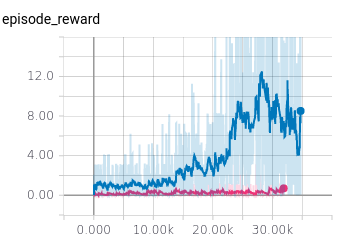
\includegraphics[scale=3]{tflearbing.png}
	  \caption{The figure shows difference of rewards achieved in case of training from scratch compared to use of transfer learning and curriculum learning. Pink - training form scratch. Blue- Transfer learning and Curriculum learning. }
	\end{figure*}

	\subsection{Curriculum Learning}
	The main concept of curriculum learning based on the fact that humans learn effectively when examples are presented in a structured manner instead of random. This strategy allows reinforcement learning agents to learn in a similar manner. The agents are represented by a task that becomes more and more complex over the course of training, with a final goal to be the intended most complex task. This leads to reduced training time because initial search space is reduced a lot. This also allows the agent to stuck in local minima. Now, we will detail how this technique helped us to train our snake agent.

	The multiplayer snake environment is complex as described above. We also state the challenges that we faced while training our agent directly in a full complex setting. These challenges were where avoided using curriculum learning.For our snake environment, we trained a single snake in a fixed window with multiple food items. Then, we used the weights of the neural network there to train the agent on a bigger field with floating window. Then, these snakes were left in a multiplayer game so that they can learn strategies related to a multiplayer gameplay. They were able to learn various strategies. We will have a look at this in the result section.


	In conclusion, Curriculum learning and transfer learning makes sense in case of Deep reinforce learning as training is online and weight sharing is a very commonly used strategy is Deep learning. These techniques are necessary for convergence an optimal solution in our snake environment. These techniques allow agents to learn more complex behaviour like avoiding each other and attacking in a competitive and cooperative setting.
	
	\subsection{Additional Ideas}
	
	
	\section{Results And Discussion}
	\begin{figure}[]

		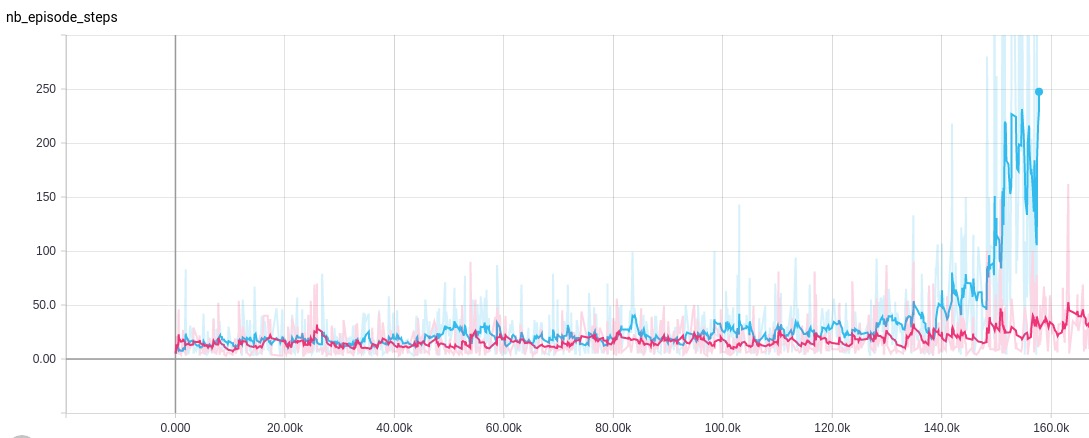
\includegraphics[width=\linewidth]{ep_step.jpeg}
		\caption{Number of steps per Episode for single player}
		\label{step}

	\end{figure}
	\begin{figure}[]

		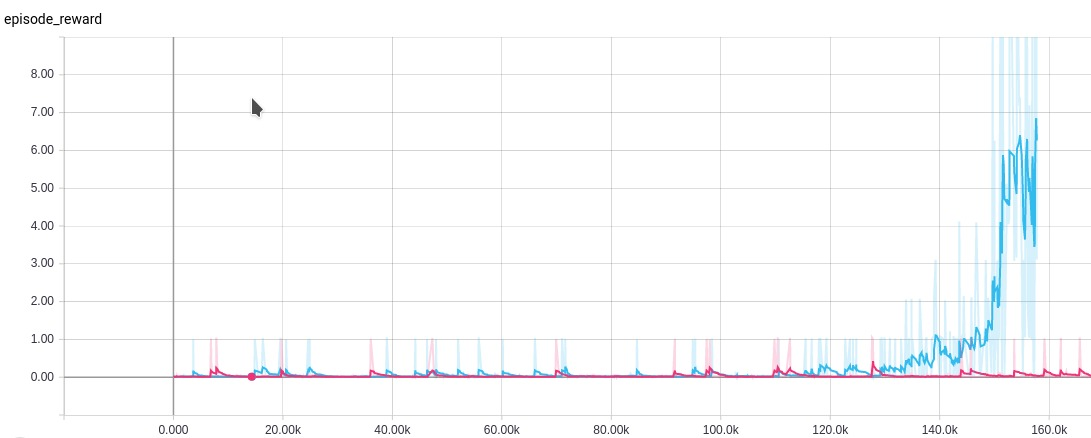
\includegraphics[width = \linewidth]{ep_reward.jpeg}
		\caption{Rewards per episode for single player}
		\label{reward}

	\end{figure}
	\subsection{Experimental Setup}
	The algorithms and the game environment were coded using python (using Keras, tensorflow and pygame libraries). The code was downloaded into a azure server and executed on it after setting up required configurations. We used a standard NC6 azure server with Nvidia K80 GPUs. The server run on linux. 
	\break
	\break
	The algorithm were run for 3 million steps and the reward and other logs were recorded.We saved weights for our agents at every 2,50,000 steps. This was done to analyze agent performance at various stages of learning.
	\subsection{How To Train}
	
	Before running the scripts, along with Python3, Tensorflow, Keras and OpenAI Gym should be installed. The code can be downloaded from our github repository\cite{code}.
	
	To train the network run
	\break
	\break
	\textit{python dqn\_snake.py --mode=train --env-name=<env-name}
	\break
	\break
	And to test it
	\break
	\break
	\textit{ python dqn\_snake.py --mode=test --env-name=env-name --weights= weights-file}
	

	\subsection{Results}
	
	\begin{figure}[]
		
		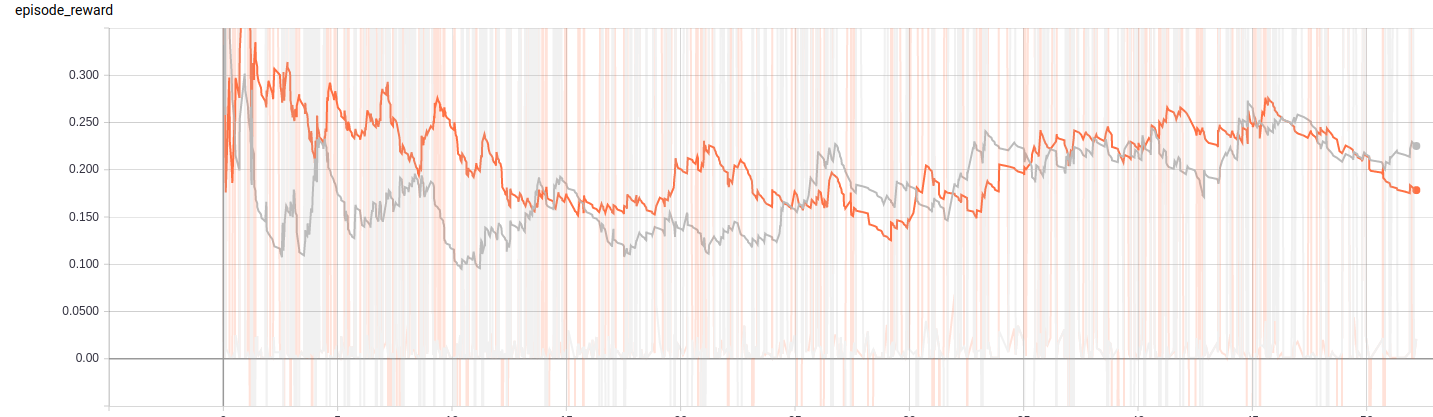
\includegraphics[width = \linewidth]{plot/snake_comp_reward.png}
		\caption{Competitive Snakes Reward Plot}
		\label{rcms}
		
	\end{figure}
	\begin{figure}[]
		
		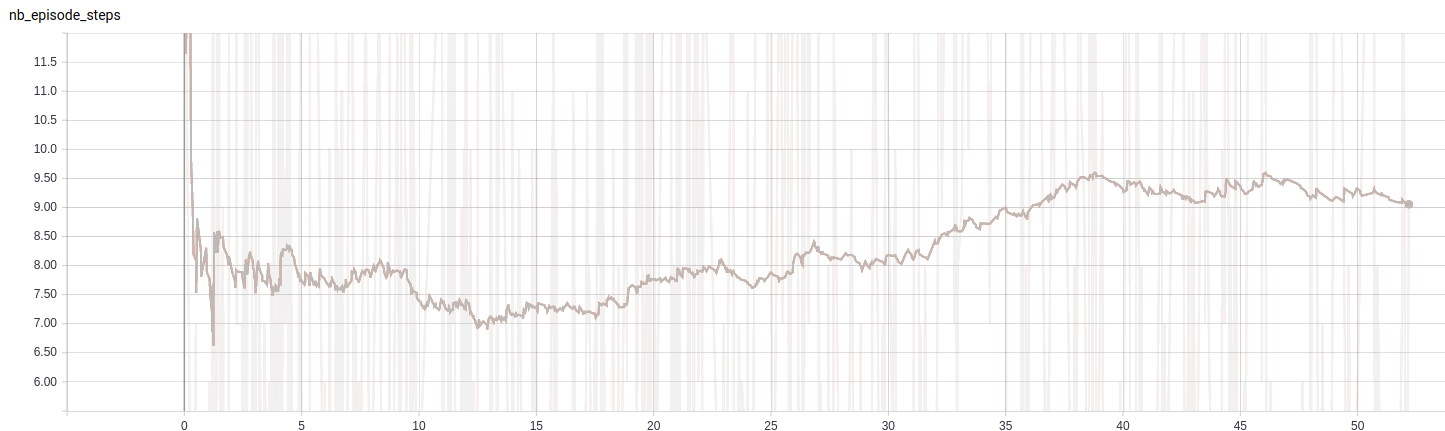
\includegraphics[width = \linewidth]{plot/snake_comp_step.png}
		\caption{Step vs. Episode Plot for competitive snake}
		\label{scms}
		
	\end{figure}
	\begin{figure}[]
		
		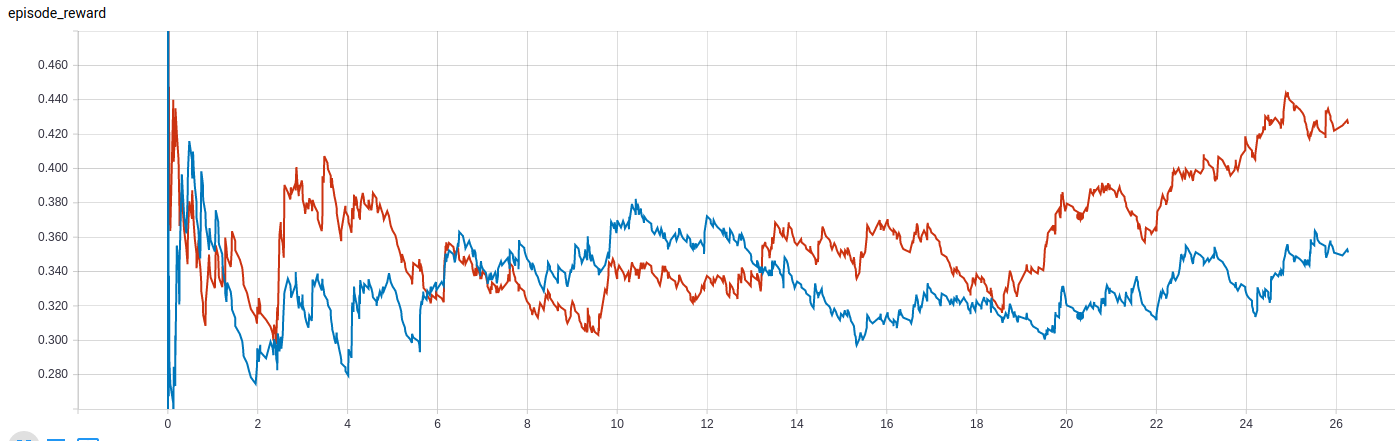
\includegraphics[width = \linewidth]{plot/snake_coop_reward.png}
		\caption{Reward Plot for a cooperative}
		\label{rcos}
		
	\end{figure}
	\begin{figure}[]
		
		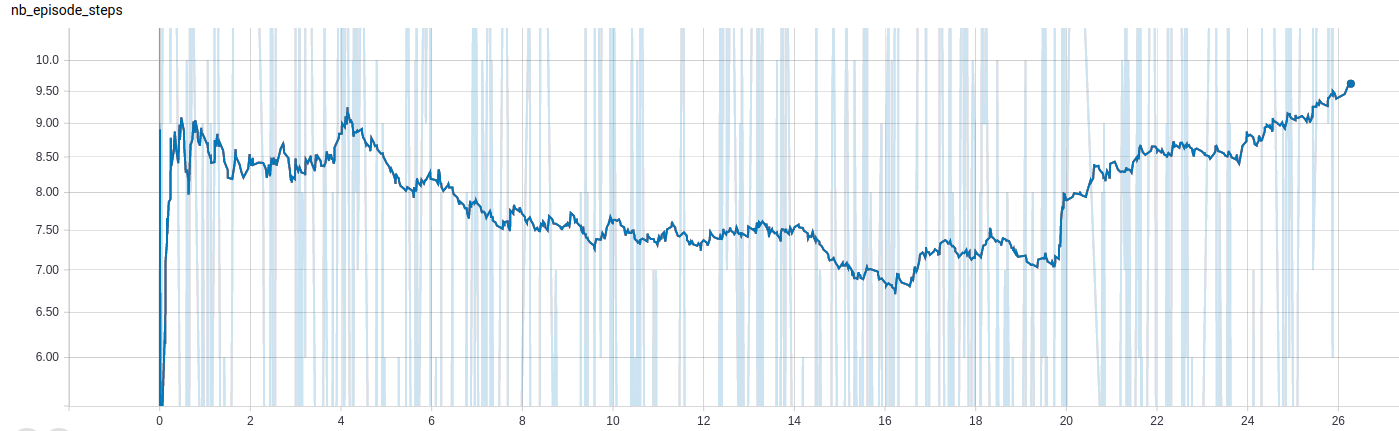
\includegraphics[width = \linewidth]{plot/snake_coop_step.png}
		\caption{Step vs. Episode plot for a cooperative Snake}
		\label{scos}
		
	\end{figure}
	\begin{figure}[]
		
		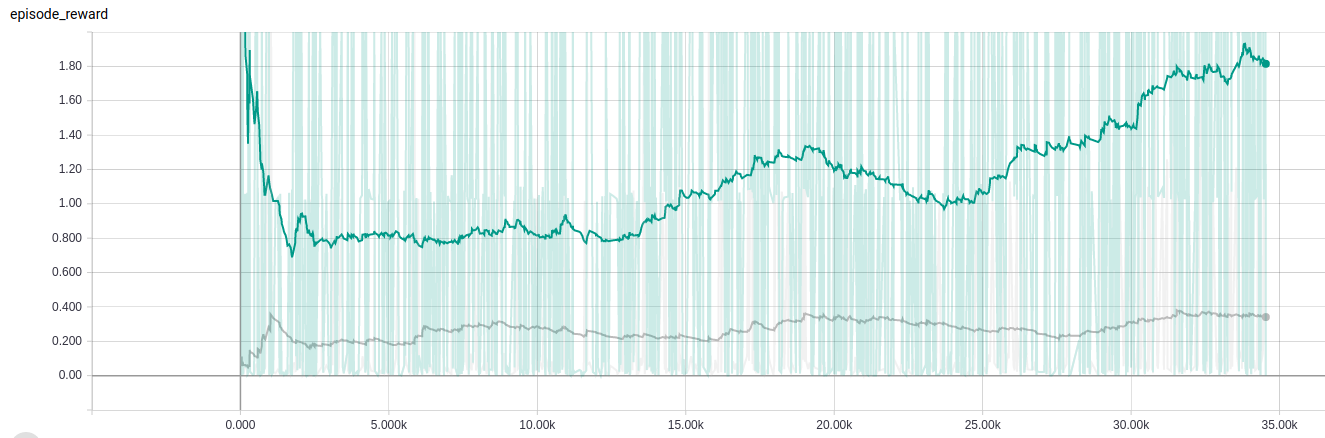
\includegraphics[width = \linewidth]{plot/snake_window_comp_reward.png}
		\caption{Reward plot for competitive  snakes in window environment}
		\label{rcmsw}
		
	\end{figure}
	\begin{figure}[]
		
		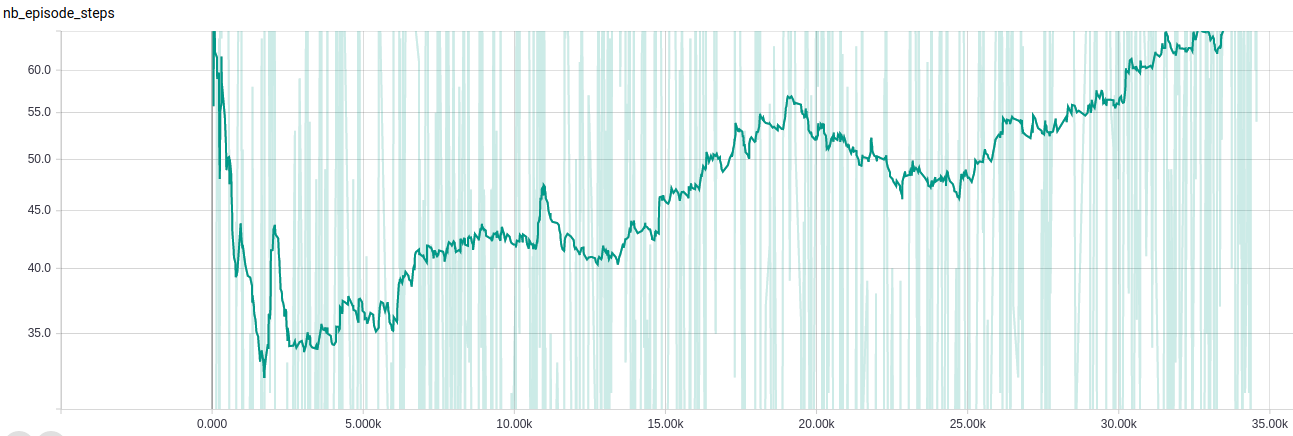
\includegraphics[width = \linewidth]{plot/snake_window_comp_step.png}
		\caption{Reward plot for competitive  snakes in window environment}
		\label{scmsw}
		
	\end{figure}\begin{figure}[]
	
	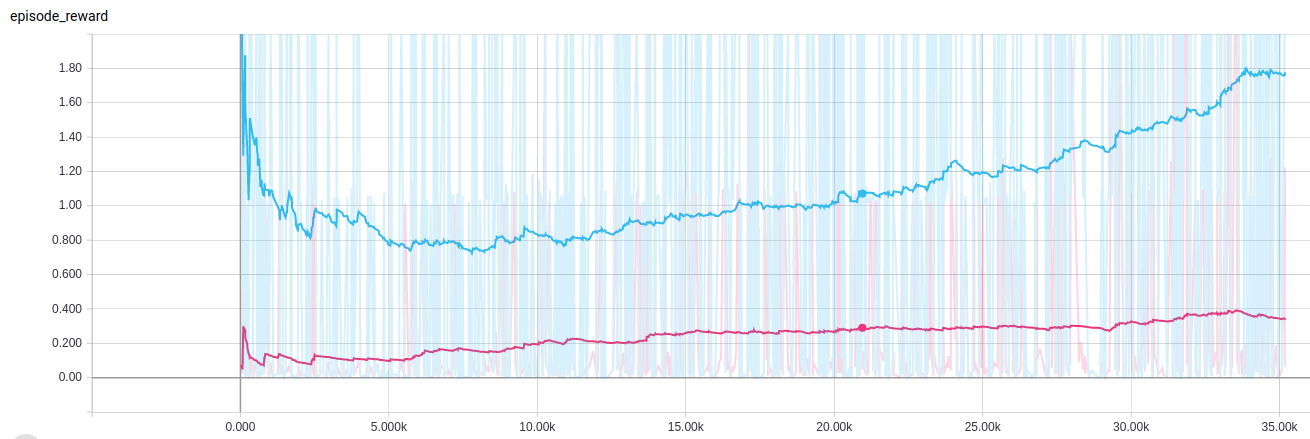
\includegraphics[width = \linewidth]{plot/snake_window_coop_reward.png}
	\caption{Reward plot for competitive  snakes in window environment}
	\label{rcosw}
	
\end{figure}\begin{figure}[]

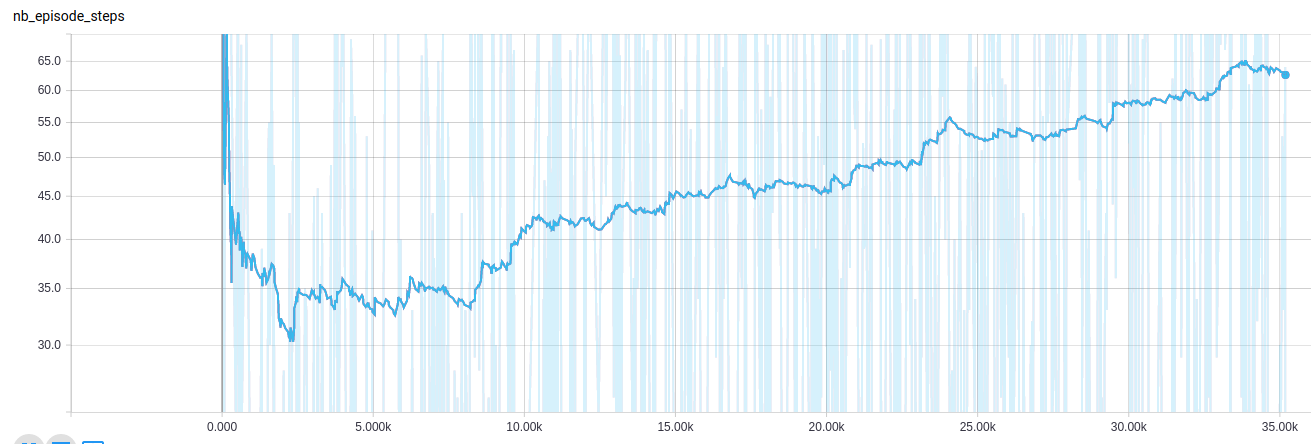
\includegraphics[width = \linewidth]{plot/snake_window_coop_step.png}
\caption{Reward plot for competitive  snakes in window environment}
\label{scosw}

\end{figure}
	Logs for the execution were monitored using Tensorboard library. Tensorboard is developed as a wrapper for Tensorflow and works with Keras library for monitoring performance of the training process.
	\break
	\break
	As can be seen from Figures as the number of steps in training continued to increase the reward obtained after each step also increased significantly.
	\break
	\break
	From the figures with single plots, it shows that the number of steps per episode increases with training. This implies that as the training continues the snake is learning to stay alive for a longer durations than before.

	\subsection{Observations}
	We would like to discuss some interesting patterns that we observed the agent learning. In single player, Initially, an agent acts randomly and most of the games end by the agent hitting itself. By 125 thousand steps, the agent learns to avoid hitting itself and moves mostly in a straight line. At this point, most games end by agent hitting the boundary wall. By 325 thousand steps,  the agent learns to avoid hitting the wall by just moving in a loop. This is a good temporary strategy, but the agent is not receiving a significant reward. So in just 50 thousand steps more, it learns to break out of the loop and chase foods. The game length is short at this point due to collisions with walls and itself in attempt to eat food. The overall performance further improves as we give our agent more time to train.
	\break
	\break
	In the multiplayer, as the training increases, the snakes learn to not hit each other and die.

\section{Conclusion}
In this project we have implemented explored reinforcement learning and applied to multi player game environments. The environment is able to learn just from the image inputs. Thus it is a powerful tool going ahead in the field of deep learning.

We first experimented with single player environemnts like ball paddle game, single player snake game etc. We used the Keras-RL library to implemet DQN algorithm. We then developed environments for multi player snake and extended the Keras-RL library for multi-agent scenario. With reinforcement learning the agent learned to play and avoid obstacles.

\section{Team Coordination}
\begin{itemize}

	\item Development of Environment: Sourav Dutta:80\%, Srajan Paliwal:10\%, Nitish Rath:10\%
	\item Single-agent Algortihm: Sourav Dutta:10\%, Srajan Paliwal:80\%, Nitish Rath:10\%
\item	Multi-agent Algorithm : Sourav Dutta:5\%, Srajan Paliwal:20\%, Nitish Rath:75\%  

\end{itemize}
\begin{thebibliography}{00}
\bibitem{sp1} Watkins, C.J. and Dayan, P., 1992. Q-learning. Machine learning, 8(3-4), pp.279-292.
\bibitem{sp2} Tan, M., 1993. Multi-agent reinforcement learning: Independent vs. cooperative agents. In Proceedings of the tenth international conference on machine learning (pp. 330-337).
\bibitem{sp3} Mnih, V., Kavukcuoglu, K., Silver, D., Graves, A., Antonoglou, I., Wierstra, D. and Riedmiller, M., 2013. Playing atari with deep reinforcement learning. arXiv preprint arXiv:1312.5602.
\bibitem{sp4} Van Hasselt, H., Guez, A. and Silver, D., 2016, February. Deep Reinforcement Learning with Double Q-Learning. In AAAI (Vol. 16, pp. 2094-2100).
\bibitem{sp5} Schaul, T., Quan, J., Antonoglou, I. and Silver, D., 2015. Prioritized experience replay. arXiv preprint arXiv:1511.05952.
\bibitem{sp6} Wang, Z., Schaul, T., Hessel, M., Van Hasselt, H., Lanctot, M. and De Freitas, N., 2015. Dueling network architectures for deep reinforcement learning. arXiv preprint arXiv:1511.06581.
\bibitem{sp7} Silver, D., Huang, A., Maddison, C.J., Guez, A., Sifre, L., Van Den Driessche, G., Schrittwieser, J., Antonoglou, I., Panneershelvam, V., Lanctot, M. and Dieleman, S., 2016. Mastering the game of Go with deep neural networks and tree search. nature, 529(7587), pp.484-489.
\bibitem{sp8} Silver, D., Schrittwieser, J., Simonyan, K., Antonoglou, I., Huang, A., Guez, A., Hubert, T., Baker, L., Lai, M., Bolton, A. and Chen, Y., 2017. Mastering the game of go without human knowledge. Nature, 550(7676), p.354.
\bibitem{sp9} Bansal, T., Pachocki, J., Sidor, S., Sutskever, I. and Mordatch, I., 2017. Emergent complexity via multi-agent competition. arXiv preprint arXiv:1710.03748.
\bibitem{sd5} Qicheng Ma, Hadon Nash, ``Solving Multiplayer Games with Reinforcement Learning,".
\bibitem{sd1} G. Brockman, V. Cheung, L. Pettersson, J. Schneider, J. Schulman, J. Tang, and W. Zaremba. OpenAI Gym. arXiv preprint arXiv:1606.01540, 2016.
\bibitem{sp10} OpenAI. (August 2017). Dota 2. [online] Available at: https://blog.openai.com/dota-2/ [Accessed 1 Feb. 2018].
\bibitem{sd2} Slither.io [online] Available at: http://slither.io/ [Accessed 1 Feb. 2018].
\bibitem{sd3}https://github.com/openai/gym
\bibitem{sd4}https://github.com/Loonride/slither.io-clone
\bibitem{n2} TensorFlow [online] Available at: https://www.tensorflow.org [Accessed 1 Feb. 2018].
\bibitem{n3} OpenAI Blog [online] Available at: https://blog.openai.com/requests-for-research-2/ [Accessed 1 Feb. 2018].
\bibitem{n4}https://arxiv.org/abs/1312.5602
\bibitem{n5}https://github.com/keras-rl/keras-rl
\bibitem{code}https://github.com/bde-slither/
\bibitem{sd7}Ardi Tampuu, Tambet Matiisen, Dorian Kodelja, Ilya Kuzovkin, Kristjan Korjus, Juhan Aru, Jaan Aru, Raul Vicente, ``Multiagent Cooperation and Competition with Deep Reinforcement Learning".

\end{thebibliography}

\end{document}
